\documentclass[14pt]{extarticle}
\usepackage[utf8]{inputenc}
\usepackage[russian]{babel}
\usepackage{indentfirst}
\usepackage{graphicx}
\usepackage{amsfonts}
\usepackage[top=2cm, bottom=2.5cm, left=2.5cm, right=2.5cm]{geometry} % Adjust margins
\usepackage{amsmath,physics}
\usepackage{tocloft}
\usepackage{tikz}
\usepackage{wrapfig}
\usepackage{float}
\usepackage{soul}
\usepackage{xcolor}
\usepackage{circledsteps}
\usepackage{colortbl}
\usetikzlibrary{shapes.geometric}
\usepackage{verbatim}
\usepackage{multicol}
\usetikzlibrary{graphs}
\usetikzlibrary{tikzmark,overlay-beamer-styles}
\usetikzlibrary{arrows}

\renewcommand\cftsecfont{\normalfont}
\renewcommand\cftsecpagefont{\normalfont}
\renewcommand{\cftsecleader}{\cftdotfill{\cftsecdotsep}}
\renewcommand\cftsecdotsep{\cftdot}
\renewcommand\cftsubsecdotsep{\cftdot}

\begin{document}

\begin{center}
Министерство образования и науки Российской Федерации\\
Федеральное государственное бюджетное образовательное учреждение\\
высшего образования\\
\textbf{«Московский авиационный институт\\
(Национальный исследовательский университет)»\\
(МАИ)}\\
Институт №8 «Компьютерные науки и прикладная математика»\\
Кафедра 806 «Прикладная математика и информатика»
\end{center}

\vspace{4cm}

\begin{center}
\textbf{КУРСОВАЯ РАБОТА}\\
по дисциплине «Дискретная математика»\\
\end{center}

\begin{center}
2 семестр\\
Вариант 11\\
\end{center}

\vspace{2cm}

\begin{flushright}
Студент: Ермеков Г.А.\\
Группа: М8О-101Б-23\\
Преподаватель: Смерчинская С. О.\\
Оценка: \underline{\hspace{3cm}}\\
Дата: \underline{\hspace{3cm}}
\end{flushright}

\vfill

\begin{center}
Москва 2024
\end{center}

\newpage

\section*{\centering ЗАДАНИЕ 1}

\textbf{Дано:} орграф, заданный матрицей смежности:
\[
A = \begin{pmatrix}
0 & 1 & 0 & 0 \\
1 & 0 & 1 & 0 \\
0 & 1 & 0 & 0 \\
1 & 1 & 1 & 0
\end{pmatrix}
\]

\textbf{Найти:} 
\begin{enumerate}
    \item матрицу односторонней связности;
    \item матрицу сильной связности;
    \item компоненты сильной связности;
    \item матрицу контуров.
\end{enumerate}

\textbf{Решение:} 
\textbf{a)} Первый способ: Алгоритм Уоршалла.
\[
T = E \lor A \lor A^2 \lor A^3:
\]
\[
A^2 = \begin{pmatrix}
1 & 0 & 1 & 0 \\
0 & 1 & 0 & 0 \\
1 & 0 & 1 & 0 \\
1 & 1 & 1 & 0
\end{pmatrix}, \quad
A^3 = \begin{pmatrix}
0 & 1 & 0 & 0 \\
1 & 0 & 1 & 0 \\
0 & 1 & 0 & 0 \\
1 & 1 & 1 & 0
\end{pmatrix}
\]
\[
T = \begin{pmatrix}
1 & 0 & 0 & 0 \\
0 & 1 & 0 & 0 \\
0 & 0 & 1 & 0 \\
0 & 0 & 0 & 1
\end{pmatrix}
\lor
\begin{pmatrix}
0 & 1 & 0 & 0 \\
1 & 0 & 1 & 0 \\
0 & 1 & 0 & 0 \\
1 & 1 & 1 & 0
\end{pmatrix}
\lor
\begin{pmatrix}
1 & 0 & 1 & 0 \\
0 & 1 & 0 & 0 \\
1 & 0 & 1 & 0 \\
1 & 1 & 1 & 0
\end{pmatrix}
\lor
\begin{pmatrix}
0 & 1 & 0 & 0 \\
1 & 0 & 1 & 0 \\
0 & 1 & 0 & 0 \\
1 & 1 & 1 & 0
\end{pmatrix}
=
\begin{pmatrix}
1 & 1 & 1 & 0 \\
1 & 1 & 1 & 0 \\
1 & 1 & 1 & 0 \\
1 & 1 & 1 & 1
\end{pmatrix}
\]
\[
T \text{--- матрица односторонней связности}
\]

\textbf{Второй способ: Итерационный алгоритм Уоршалла.}
\[
T^{(0)} = E \lor A = \begin{pmatrix}
1 & 0 & 0 & 0 \\
0 & 1 & 0 & 0 \\
0 & 0 & 1 & 0 \\
0 & 0 & 0 & 1
\end{pmatrix}
\lor
\begin{pmatrix}
0 & 1 & 0 & 0 \\
1 & 0 & 1 & 0 \\
0 & 1 & 0 & 0 \\
1 & 1 & 1 & 0
\end{pmatrix}
=
\begin{pmatrix}
1 & 1 & 0 & 0 \\
1 & 1 & 1 & 0 \\
0 & 1 & 1 & 0 \\
1 & 1 & 1 & 1
\end{pmatrix}
\]

\[
T^{(1)} = \begin{pmatrix}
1 & 1 & 0 & 0 \\
1 & 1 & 1 & 0\\
0 & 1 & 1 & 0\\
1 & 1 & 1 & 1
\end{pmatrix}
\lor
\begin{pmatrix}
1 & 1 & 0 & 0 \\
1 & 1 & 0 & 0 \\
0 & 0 & 0 & 0 \\
1 & 1 & 0 & 0
\end{pmatrix}
= 
\begin{pmatrix}
1 & 1 & 0 & 0 \\
1 & 1 & 1 & 0 \\
0 & 1 & 1 & 0 \\
1 & 1 & 1 & 1
\end{pmatrix}
\]

\[
T^{(2)} = \begin{pmatrix}
1 & 1 & 0 & 0 \\
1 & 1 & 1 & 0 \\
0 & 1 & 1 & 0 \\
1 & 1 & 1 & 1
\end{pmatrix}
\lor
\begin{pmatrix}
1 & 1 & 1 & 0 \\
1 & 1 & 1 & 0 \\
1 & 1 & 1 & 0 \\
1 & 1 & 1 & 0
\end{pmatrix}
=
\begin{pmatrix}
1 & 1 & 1 & 0 \\
1 & 1 & 1 & 0 \\
1 & 1 & 1 & 0 \\
1 & 1 & 1 & 1
\end{pmatrix}
\]

\[
T^{(3)} = \begin{pmatrix}
1 & 1 & 1 & 0 \\
1 & 1 & 1 & 0 \\
1 & 1 & 1 & 0 \\
1 & 1 & 1 & 1
\end{pmatrix}
\lor
\begin{pmatrix}
1 & 1 & 1 & 0 \\
1 & 1 & 1 & 0 \\
1 & 1 & 1 & 0 \\
1 & 1 & 1 & 0
\end{pmatrix}
=
\begin{pmatrix}
1 & 1 & 1 & 0 \\
1 & 1 & 1 & 0 \\
1 & 1 & 1 & 0 \\
1 & 1 & 1 & 1
\end{pmatrix}
\]

\[
T^{[4]} = \begin{pmatrix}
1 & 1 & 1 & 0 \\
1 & 1 & 1 & 0 \\
1 & 1 & 1 & 0 \\
1 & 1 & 1 & 1
\end{pmatrix}
\lor
\begin{pmatrix}
0 & 0 & 0 & 0 \\
0 & 0 & 0 & 0 \\
0 & 0 & 0 & 0 \\
1 & 1 & 1 & 1
\end{pmatrix}
=
\begin{pmatrix}
1 & 1 & 1 & 0 \\
1 & 1 & 1 & 0 \\
1 & 1 & 1 & 0 \\
1 & 1 & 1 & 1
\end{pmatrix}
\]
\[
T^{(4)} \text{--- матрица односторонней связности}
\]

\textbf{б)} \( \overline{S} = T \& T^T \)
\[
S = \begin{pmatrix}
1 & 1 & 1 & 0 \\
1 & 1 & 1 & 0 \\ 
1 & 1 & 1 & 0 \\
1 & 1 & 1 & 1
\end{pmatrix} \& \begin{pmatrix}
1 & 1 & 1 & 1 \\
1 & 1 & 1 & 1 \\
1 & 1 & 1 & 1 \\
0 & 0 & 0 & 1
\end{pmatrix} = \begin{pmatrix}
1 & 1 & 1 & 0 \\
1 & 1 & 1 & 0 \\
1 & 1 & 1 & 0 \\
0 & 0 & 0 & 1
\end{pmatrix}
\]

\textbf{в)} Первая компонента: \(\{v_1,v_2,v_3\}\);вторая компонента: \(\{v_4\}\)
\[
\overline{S_1} = \begin{pmatrix}
0 & 0 & 0 & 0 \\
0 & 0 & 0 & 0 \\
0 & 0 & 0 & 0 \\
0 & 0 & 0 & 1
\end{pmatrix}
\]
Обнуляем 4 столбец, получаем нулевую матрицу, след. третьих компонентов сильной связности нет.

\textbf{г)} \[ K = \overline{S} \& A = 
\begin{pmatrix}
1 & 1 & 1 & 0 \\
1 & 1 & 1 & 0 \\
1 & 1 & 1 & 0 \\
0 & 0 & 0 & 1
\end{pmatrix}
\&
\begin{pmatrix}
0 & 1 & 0 & 0 \\
1 & 0 & 1 & 0 \\
0 & 1 & 0 & 0 \\
1 & 1 & 1 & 0
\end{pmatrix}
=
\begin{pmatrix}
0 & 1 & 0 & 0 \\
1 & 0 & 1 & 0 \\
0 & 1 & 0 & 0 \\
0 & 0 & 0 & 0
\end{pmatrix}
\]
\textbf{Дуги:} <\(v_1, v_2\)>, <\(v_2, v_1\)>, <\(v_2, v_3\)>, <\(v_3, v_2\)>
\newpage
\textbf{д)} Рисунок графа:\\
\begin{center}
\begin{tikzpicture}[node distance=3cm, main/.style = {draw, circle}] 
\node[main] (1) {\(v_1\)}; 
\node[main] (2) [below right of=1] {\(v_2\)}; 
\node[main] (3) [below left of=2] {\(v_3\)}; 
\node[main] (4) [below left of=1] {\(v_4\)}; 

\draw[->] (1) to [out=-20, in=110, looseness=1] (2);
\draw[->] (2) to [out=160, in=-70, looseness=1] (1);
\draw[->] (3) to [out=20, in=-110, looseness=1] (2);
\draw[->] (2) to [out=-160, in=70, looseness=1] (3);
\draw[->] (4) -> (1)
\draw[->] (4) -> (2)
\draw[->] (4) -> (3)
\end{tikzpicture} 
\end{center}

\section*{\centering ЗАДАНИЕ 2}
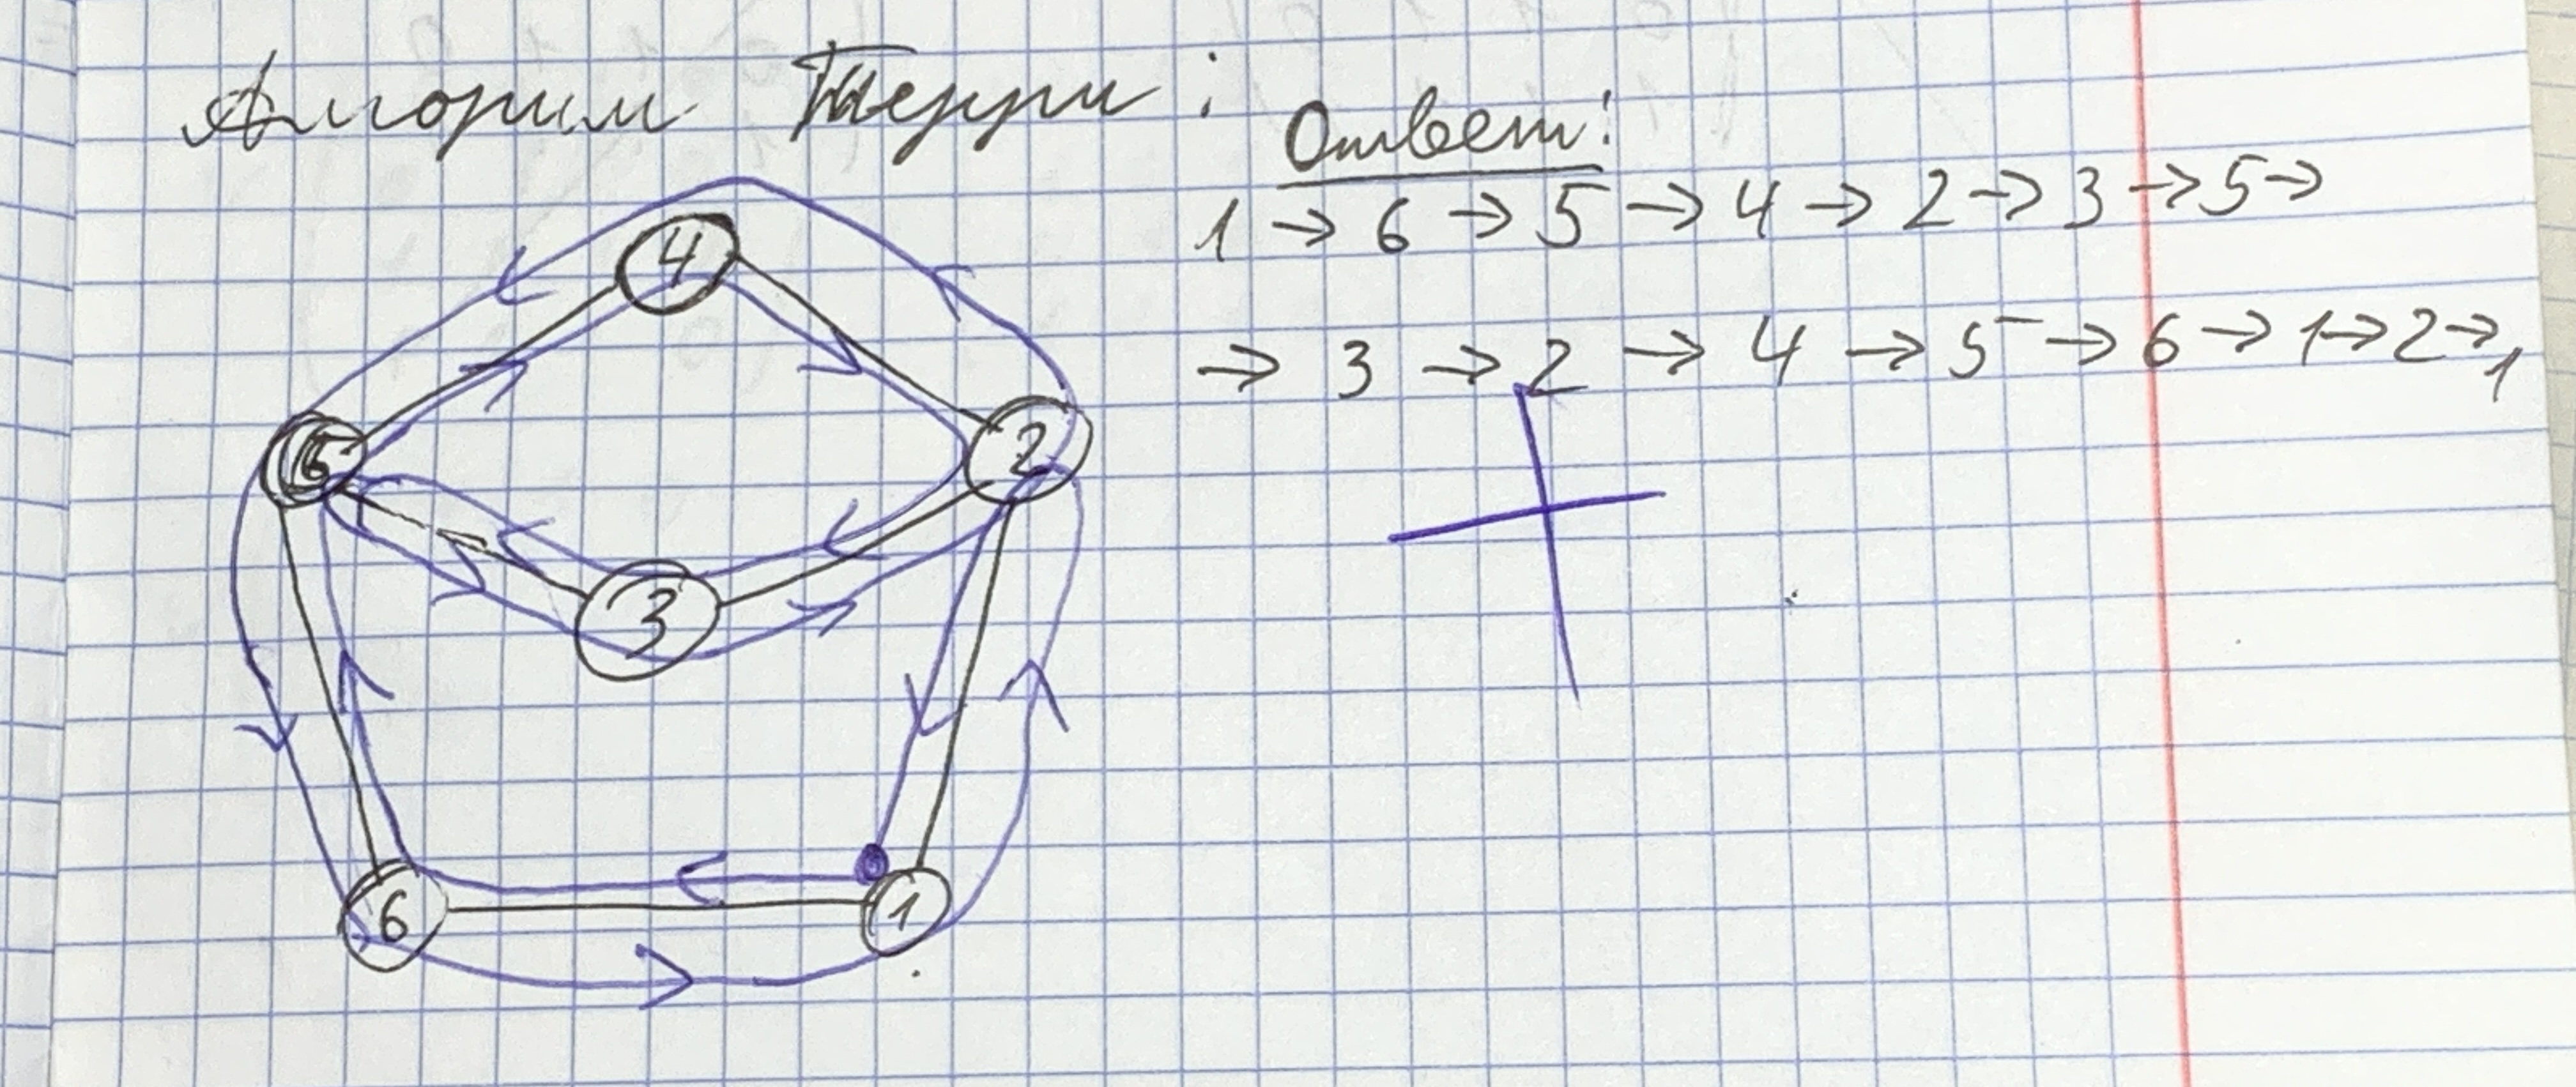
\includegraphics[width=1\linewidth]{2.jpg}

\section*{\centering ЗАДАНИЕ 3}
\[
\centering
A = \begin{pmatrix}
0 & 0 & 0 & 1 & 0 & 1 & 0 \\
1 & 0 & 1 & 0 & 1 & 0 & 1 \\
0 & 1 & 0 & 1 & 1 & 1 & 0 \\
1 & 0 & 0 & 0 & 1 & 0 & 0 \\
1 & 0 & 1 & 1 & 0 & 1 & 0 \\
0 & 0 & 0 & 1 & 1 & 0 & 0 \\
1 & 0 & 1 & 0 & 1 & 1 & 0
\end{pmatrix}
\]



\begin{minipage}{0.55\textwidth}
\begin{tikzpicture}[node distance=3cm, main/.style = {draw, circle}] 
\node[main] (1) {\(v_1\)}; 
\node[main] (2) [below right of=1] {\(v_6\)}; 
\node[main] (3) [below left of=1] {\(v_4\)}; 
\node[main] (4) [below left of=2] {\(v_5\)}; 
\node[main] (5) [below of=4] {\(v_3\)}; 
\node[main] (6) [below of=5] {\(v_2\)}; 
\node[main] (7) [below of=6] {\(v_7\)}; 

\draw[->] (1) -> (2);
\draw[->] (1) -> (3);
\draw[->] (2) -> (4);
\draw[->] (3) -> (4);
\draw[->] (4) -> (5)
\draw[->] (5) -> (6)
\draw[->] (6) -> (7)
\end{tikzpicture} 
\end{minipage}
\begin{minipage}{0.4\textwidth}
    \[Fw_0 = \{v_1\}\]
    \vspace{1.3cm}
    \[Fw_1 = \{v_4, v_6\}\]
    \vspace{1.3cm}
    \[Fw_2 = \{v_5\}\]
    \vspace{1.3cm}
    \[Fw_3 = \{v_3\}\]
    \vspace{1.3cm}
    \[Fw_4 = \{v_2\}\]
    \vspace{1.3cm}
    \[Fw_5 = \{v_7\}\]
    \vspace{0.01cm}
    
\end{minipage}
\\
\textbf{1)} \(v_7\)\\
\textbf{2)} \(w_4(v_1) \bigcap F^{-1}v_7 = \{v_2\} \bigcap \{v_2\} = \{v_2\}\)\\
\textbf{3)} \(w_3(v_1) \bigcap F^{-1}v_2 = \{v_3\} \bigcap \{v_3\} = \{v_3\}\)\\
\textbf{4)} \(w_2(v_1) \bigcap F^{-1}v_3 = \{v_5\} \bigcap \{v_2, v_5, v_7\} = \{v_5\}\)\\
\textbf{5)} \(w_1(v_1) \bigcap F^{-1}v_5 = \{v_4, v_6\} \bigcap \{v_2, v_3, v_4, v_6, v_7\} = \{v_4, v_6\}\)\\
\textbf{6.1)} \(w_0(v_1) \bigcap F^{-1}v_4 = \{v_1\} \bigcap \{v_1, v_3, v_5, v_6\} = \{v_1\}\)\\
\textbf{6.2)} \(w_0(v_1) \bigcap F^{-1}v_6 = \{v_1\} \bigcap \{v_1, v_3, v_5, v_7\} = \{v_1\}\) \\

\textbf{Кратчайшие пути:}\\
\[v_1 - v_4 - v_5 - v_3 - v_2 - v_7\]
\[v_1 - v_6 - v_5 - v_3 - v_2 - v_7\]

\newpage
\section*{\centering ЗАДАНИЕ 4}
Составим таблицу итераций:
\begin{center}
		\begin{tabular}{|c|c|c|c|c|c|c|c|c|c|c|c|c|c|c|c|c|}
			\hline 
			$ $& $V_1$ & $V_2$ & $V_3$ & $V_4$ & $V_5$ & $V_6$ & $V_7$ & $V_8$ & $\lambda_i^{(0)}$ & $\lambda_i^{(1)}$ & $\lambda_i^{(2)}$ & $\lambda_i^{(3)}$ & $\lambda_i^{(4)}$ & $\lambda_i^{(5)}$ & $\lambda_i^{(6)}$ & $\lambda_i^{(7)}$ \\ \hline
			
			$V_1$ & $\infty$ & 2 & $\infty$ & 5 & $\infty$ & 6 & $\infty$ & $\infty$ & \tikzmarknode{m1}{\Circled{0}} & 0 & 0 & 0 & 0 & 0 & 0 & 0\\ \hline
			
			$V_2$ & 6 & $\infty$ & 12 & 3 & $\infty$ & $\infty$ & $\infty$ & $\infty$ & $\infty$ & \tikzmarknode{m2}{\Circled{2}} & 2 & 2 & 2 & 2 & 2 & 2\\ \hline
			
			$V_3$ & 7 & $\infty$ & $\infty$ & $\infty$ & 1 & $\infty$ & $\infty$ & 1 & $\infty$ & $\infty$ & 14 & 12 & \tikzmarknode{m3}{\Circled{12}} & 12 & 12 & 12\\ \hline
			
			$V_4$ & 5 & 3 & $\infty$ & $\infty$ & 6 & 2 & $\infty$ & $\infty$ & $\infty$ & 5 & \tikzmarknode{m4}{\Circled{5}} & 5 & 5 & 5 & 5 & 5 \\ \hline
			
			$V_5$ & $\infty$ & $\infty$ & 1 & $\infty$ & $\infty$ & $\infty$ & 3 & 4 & $\infty$ & $\infty$ & 11 & \tikzmarknode{m5}{\Circled{11}} & 11 & 11 & 11 & 11\\ \hline
			
			$V_6$ & 3 & $\infty$ & $\infty$ & 2 & $\infty$ & $\infty$ & 2 & $\infty$ & $\infty$ & \tikzmarknode{m6}{\Circled{6}} & 6 & 6 & 6 & 6 & 6 & 6 \\ \hline
			
			$V_7$ & $\infty$ & $\infty$ & $\infty$ & $\infty$ & 3 & $\infty$ &  $\infty$ & 6 & $\infty$ & $\infty$ & \tikzmarknode{m7}{\Circled{8}} & 8 & 8 & 8 & 8 & 8 \\ \hline
			
			$V_8$ & 8 & $\infty$ & $\infty$ & $\infty$ & 13 & $\infty$ & $\infty$ &  $\infty$ & $\infty$ & $\infty$ & $\infty$ & 14 & 13 & \tikzmarknode{m8}{\Circled{13}} & 13 & 13 \\ \hline

	\end{tabular}
\end{center}
\begin{tikzpicture}[remember picture,overlay]
\draw[->] (m1) -- (m2);
\draw[->] (m2) -- (m4);
\draw[->] (m4) -- (m5);
\draw[->] (m5) -- (m3);
\draw[->] (m1) -- (m6);
\draw[->] (m6) -- (m7);
\draw[->] (m3) -- (m8);
\end{tikzpicture}
\textbf{Пути:}\\
\begin{enumerate}
    \item \(min &: v_1 \xrightarrow{} v_2 = 2\)\\
    \(\lambda_1^{(0)} + c_1_2 &= 0+2 &= 2 &= \lambda_2^{(1)}\)
    
    \item \(min &: v_1 \xrightarrow{} v_3 = 12\)\\
    \(\lambda_1^{(0)} + c_1_2 &= 0+2 &= 2 &= \lambda_2^{(1)}\)
    \(\lambda_2^{(1)} + c_2_4 &= 2+3 &= 5 &= \lambda_4^{(2)}\)\\
    \(\lambda_4^{(2)} + c_4_5 &= 5+6 &= 11 &= \lambda_5^{(3)}\)\\
    \(\lambda_5^{(3)} + c_5_3 &= 1+11 &= 12 &= \lambda_3^{(4)}\)
    
    \item \(min &: v_1 \xrightarrow{} v_4 = 5\)\\
    \(\lambda_1^{(0)} + c_1_2 &= 0+2 &= 2 &= \lambda_2^{(1)}\)\\
    \(\lambda_2^{(1)} + c_2_4 &= 2+3 &= 5 &= \lambda_4^{(2)}\)
    
    \item \(min &: v_1 \xrightarrow{} v_5 = 6\)\\
    \(\lambda_1^{(0)} + c_1_2 &= 0+2 &= 2 &= \lambda_2^{(1)}\)\\
    \(\lambda_2^{(1)} + c_2_4 &= 2+3 &= 5 &= \lambda_4^{(2)}\)\\
    \(\lambda_4^{(2)} + c_4_5 &= 5+6 &= 11 &= \lambda_5^{(3)}\)
    
    \item \(min &: v_1 \xrightarrow{} v_6 = 6\)\\
    \(\lambda_1^{(0)} + c_1_6 &= 0+6 &= 6 &= \lambda_6^{(1)}\)
    
    \item \(min &: v_1 \xrightarrow{} v_7 = 8\)\\
    \(\lambda_1^{(0)} + c_1_6 &= 0+6 &= 6 &= \lambda_6^{(1)}\)\\
    \(\lambda_6^{(1)} + c_7_6 &= 6+2 &= 8 &= \lambda_7^{(2)}\)
    
    \item \(min &: v_1 \xrightarrow{} v_8 = 14\)\\
    \(\lambda_1^{(0)} + c_1_2 &= 0+2 &= 2 &= \lambda_2^{(1)}\)
    \(\lambda_2^{(1)} + c_2_4 &= 2+3 &= 5 &= \lambda_4^{(2)}\)\\
    \(\lambda_4^{(2)} + c_4_5 &= 5+6 &= 11 &= \lambda_5^{(3)}\)\\
    \(\lambda_5^{(3)} + c_5_3 &= 1+11 &= 12 &= \lambda_3^{(4)}\)
    \(\lambda_3^{(4)} + c_3_8 &= 12+1 &= 13 &= \lambda_8^{(5)}\)
    

\textbf{Минимальные пути:}
\begin{multicols}{2}
    \[v_1 \xrightarrow{} v_2 &= 2\]
    \[v_1 \xrightarrow{} v_4 \xrightarrow{} v_5 \xrightarrow{} v_3 &= 12\]
    \[v_1 \xrightarrow{} v_4 &= 5\]
    \[v_1 \xrightarrow{} v_4 \xrightarrow{} v_5 &= 11\]
    \[v_1 \xrightarrow{} v_6 &= 6\]
    \[v_1 \xrightarrow{} v_6 \xrightarrow{} v_7 &= 8\]
    \[v_1 \xrightarrow{} v_6 \xrightarrow{} v_7 \xrightarrow{} v_8 &= 14\]
\end{multicols}
\end{enumerate}
\newpage

\section*{\centering ЗАДАНИЕ 5}
\begin{center}
	\begin{tikzpicture}
		\tikzset{vertex/.style = {shape=circle, fill, draw, minimum size=1em}}
  \tikzset{edge/.style = {draw, thick, ->}}
  % Вершины
  \node[vertex] (1) at (0,0);
  \node[vertex] (2) at (2,0);
  \node[vertex] (3) at (4,0);
  \node[vertex] (4) at (6,0);
  \node[vertex] (5) at (0,-2);
  \node[vertex] (6) at (2,-2);
  \node[vertex] (7) at (4,-2);
  \node[vertex] (8) at (6,-2);
  \node[vertex] (9) at (0,-4);
  \node[vertex] (10) at (2,-4);
  \node[vertex] (11) at (4,-4);
  \node[vertex] (12) at (6,-4);

  % Рёбра
  \draw (1) -- (2) node[midway, fill=white] {2};
  \draw (2) -- (3) node[midway, fill=white] {2};
  \draw (3) -- (4) node[midway, fill=white] {4};
  \draw (1) -- (5) node[midway, fill=white] {4};
  \draw (2) -- (6) node[midway, fill=white] {5};
  \draw (3) -- (7) node[midway, fill=white] {5};
  \draw (4) -- (8) node[midway, fill=white] {8};
  \draw (5) -- (6) node[midway, fill=white] {1};
  \draw (6) -- (7) node[midway, fill=white] {6};
  \draw (7) -- (8) node[midway, fill=white] {3};
  \draw (5) -- (9) node[midway, fill=white] {3};
  \draw (6) -- (10) node[midway, fill=white] {5};
  \draw (7) -- (11) node[midway, fill=white] {5};
  \draw (8) -- (12) node[midway, fill=white] {7};
  \draw (9) -- (10) node[midway, fill=white] {5};
  \draw (10) -- (11) node[midway, fill=white] {7};
  \draw (11) -- (12) node[midway, fill=white] {6};
\end{tikzpicture} 
\end{center}\\
\hspace{6mm}Возможное остовное дерево с минимальной суммой длин ребер:
\begin{center}
	\begin{tikzpicture}
		\tikzset{vertex/.style = {shape=circle, fill, draw, minimum size=0.1cm}}
  \tikzset{edge/.style = {draw, thick, ->}}
  % Вершины
  \node[vertex] (1) at (0,0);
  \node[vertex] (2) at (2,0);
  \node[vertex] (3) at (4,0);
  \node[vertex] (4) at (6,0);
  \node[vertex] (5) at (0,-2);
  \node[vertex] (6) at (2,-2);
  \node[vertex] (7) at (4,-2);
  \node[vertex] (8) at (6,-2);
  \node[vertex] (9) at (0,-4);
  \node[vertex] (10) at (2,-4);
  \node[vertex] (11) at (4,-4);
  \node[vertex] (12) at (6,-4);

  % Рёбра
  \draw (1) -- (2) node[midway, fill=white] {2};
  \draw (2) -- (3) node[midway, fill=white] {2};
  \draw (3) -- (4) node[midway, fill=white] {4};
  \draw (1) -- (5) node[midway, fill=white] {4};
  % \draw (2) -- (6) node[midway, fill=white] {5};
  \draw (3) -- (7) node[midway, fill=white] {5};
  % \draw (4) -- (8) node[midway, fill=white] {8};
  \draw (5) -- (6) node[midway, fill=white] {1};
  % \draw (6) -- (7) node[midway, fill=white] {6};
  \draw (7) -- (8) node[midway, fill=white] {3};
  \draw (5) -- (9) node[midway, fill=white] {3};
  \draw (6) -- (10) node[midway, fill=white] {5};
  \draw (7) -- (11) node[midway, fill=white] {5};
  % \draw (8) -- (12) node[midway, fill=white] {7};
  % \draw (9) -- (10) node[midway, fill=white] {5};
  % \draw (10) -- (11) node[midway, fill=white] {7};
  \draw (11) -- (12) node[midway, fill=white] {6};
  
\end{tikzpicture} 
\end{center}\\
\hspace{6mm}Минимальный вес остовного дерева $L(D) = 40$\
\newpage
\section*{\centering ЗАДАНИЕ 6}
\textbf{Задание:} Составить ЛНЗ системы уравнений Кирхгофа тока и напряжения\\
\begin{center}
\begin{tikzpicture}[node distance=3cm, vertex/.style={circle, draw}, every edge/.style={draw}]
    \node[vertex] (1) {1};
    \node[vertex] (2) [right of=1] {2};
    \node[vertex] (6) [below left of=1] {6};
    \node[vertex] (5) [below right of=6] {5};
    \node[vertex] (3) [below right of=2] {3};
    \node[vertex] (4) [right of=5] {4};

    \draw (1) -- (5) node[midway, fill=white] {$q_7$};
    \draw (1) -- (4) node[yshift=0.8cm, fill=white] {$q_8$};
    \draw (1) -- (2) node[midway, fill=white] {$q_2$};
    \draw (1) -- (6) node[midway, fill=white] {$q_1$};
    \draw (2) -- (5) node[xshift=1cm, yshift=0.6cm, fill=white] {$q_9$};
    \draw (2) -- (3) node[midway, fill=white] {$q_6$};
    \draw (3) -- (4) node[midway, fill=white] {$q_5$};
    \draw (4) -- (5) node[midway, fill=white] {$q_4$};
    \draw (5) -- (6) node[midway, fill=white] {$q_3$};
    
\end{tikzpicture}
\end{center}

\textbf{\underline{Решение}}\\
\noindent
1. Зададим на графе произвольную ориентацию:\\
\begin{center}
\begin{tikzpicture}[node distance=3cm, vertex/.style={circle, draw}, every edge/.style={draw}]
    \node[vertex] (1) {1};
    \node[vertex] (2) [right of=1] {2};
    \node[vertex] (6) [below left of=1] {6};
    \node[vertex] (5) [below right of=6] {5};
    \node[vertex] (3) [below right of=2] {3};
    \node[vertex] (4) [right of=5] {4};

    \draw[->] (1) -> (5) node[midway, fill=white] {$q_7$};
    \draw[<-] (1) -- (4) node[yshift=0.8cm, fill=white] {$q_8$};
    \draw[->] (1) -- (2) node[midway, fill=white] {$q_2$};
    \draw[->] (1) -- (6) node[midway, fill=white] {$q_1$};
    \draw[->] (2) -- (5) node[xshift=1cm, yshift=0.6cm, fill=white] {$q_9$};
    \draw[->] (2) -- (3) node[midway, fill=white] {$q_6$};
    \draw[<-] (3) -- (4) node[midway, fill=white] {$q_5$};
    \draw[<-] (4) -- (5) node[midway, fill=white] {$q_4$};
    \draw[->] (5) -- (6) node[midway, fill=white] {$q_3$};
    
\end{tikzpicture}
\end{center}

\noindent
2. Построим произвольное остовное дерево \textbf{\textit{D}} заданного графа:\\
\begin{center}
\begin{tikzpicture}[node distance=3cm, vertex/.style={circle, draw}, every edge/.style={draw}]
    \node[vertex] (1) {1};
    \node[vertex] (2) [right of=1] {2};
    \node[vertex] (6) [below left of=1] {6};
    \node[vertex] (5) [below right of=6] {5};
    \node[vertex] (3) [below right of=2] {3};
    \node[vertex] (4) [right of=5] {4};

    \draw (1) -- (5) node[midway, fill=white] {$q_7$};
    \draw[dotted, line width=1pt, dot={3pt 5pt}] (1) -- (4) node[yshift=0.8cm, fill=white] {$q_8$};
    \draw (1) -- (2) node[midway, fill=white] {$q_2$};
    \draw[dotted, line width=1pt, dot={3pt 5pt}] (1) -- (6) node[midway, fill=white] {$q_1$};
    \draw[dotted, line width=1pt, dot={3pt 5pt}] (2) -- (5) node[xshift=1cm, yshift=0.6cm, fill=white] {$q_9$};
    \draw (2) -- (3) node[midway, fill=white] {$q_6$};
    \draw[dotted, line width=1pt, dot={3pt 5pt}] (3) -- (4) node[midway, fill=white] {$q_5$};
    \draw (4) -- (5) node[midway, fill=white] {$q_4$};
    \draw (5) -- (6) node[midway, fill=white] {$q_3$};
    
\end{tikzpicture}
\end{center}

\hspace{2cm} Ребра \(q_1 и q_5\) соответствуют ЭДС в основном\\
\noindent
3. Найдем базис циклов, добавляя по одному не вошедшему в него ребру. Затем найдем соответствующие векторные циклы.\\
$(D+q_1): \mu_1: v_1 - v_5 - v_6 - v_1 \Rightarrow C(\mu_1) &= (-1, 0, 1, 0, 0, 0, 1, 0, 0)$\\
$(D+q_8): \mu_2: v_1 - v_5 - v_4 - v_1 \Rightarrow C(\mu_2) &= (0, 0, 0, 1, 0, 0, 1, 1, 0)$\\
$(D+q_9): \mu_3: v_1 - v_2 - v_5 - v_1 \Rightarrow C(\mu_3) &= (0, 1, 0, 0, 0, 0, -1, 0, 1)$\\
$(D+q_5): \mu_4: v_1 - v_2 - v_4 - v_1 \Rightarrow C(\mu_4) &= (0, 1, 0, -1, -1, 1, -1, 0, 0)$\\

\vspace{5mm}\\ 
\noindent
4. Циклическая матрица графа имеет вид:
\vspace{5mm}
\[C = 
\begin{pmatrix}
-1 & 0 & 1 &  0 & 0 & 0 &  1 & 0 & 0\\
 0 & 0 & 0 &  1 & 0 & 0 &  1 & 1 & 0\\
 0 & 1 & 0 &  0 & 0 & 0 & -1 & 0 & 1\\
 0 & 1 & 0 & -1 &-1 & 1 & -1 & 0 & 0
\end{pmatrix}
\]
\\
\noindent
5. Выпишем закон Кирхгофа для напряжений:
\[
\begin{pmatrix}
-1 & 0 & 1 &  0 & 0 & 0 &  1 & 0 & 0\\
 0 & 0 & 0 &  1 & 0 & 0 &  1 & 1 & 0\\
 0 & 1 & 0 &  0 & 0 & 0 & -1 & 0 & 1\\
 0 & 1 & 0 & -1 &-1 & 1 & -1 & 0 & 0
\end{pmatrix}
\begin{pmatrix}
u_1\\
u_2\\
u_3\\
u_4\\
u_5\\
u_6\\
u_7\\
u_8\\
u_9
\end{pmatrix}
&= 0
\]
\noindent
\hspace{1cm}
Напряжение, соответствующее ребрам не входящих в основное древо
\(u_1, u_5, u_8, u_9\) - базисные переменные системы; остальные - свободные

\begin{minipage}{0.4\textwidth}
\begin{cases}
-u_1 + u_3 + u_7 = 0\\
u_4 + u_7 + u_8 = 0\\
u_2 - u_7 + u_9 = 0\\
u_2 - u_4 - u_5 + u_6 - u_7= 0
\end{cases}
\end{minipage}
\noindent
\hspace{1.4cm}
\begin{minipage}{0.4\textwidth}
\begin{cases}
u_1 = u_3 + u_7\\
u_8 = -u_4 - u_7\\
u_9 = u_7 - u_2\\
u_5 = u_4 - u_2 - u_6 + u_7
\end{cases}
\end{minipage}
\vspace{5mm}
\noindent
6. Выпишем уравнения Кирхгофа для токов.\\
\hspace{1cm}
Найдем матрицу инцидентности \textbf{\textit{B}} для орграфа:
\begin{center}
\begin{tabular}{|c|c|c|c|c|c|c|c|c|c|}
\hline 
$ $ & $q_1$ & $q_2$ & $q_3$ & $q_4$ & $q_5$ & $q_6$ & $q_7$ & $q_8$ & $q_9$ \\ \hline
$v_1$ & -1 & -1 & 0 & 0 & 0 & 0 & -1 & 1 & 0 \\ \hline
$v_2$ & 0 & 1 & 0 & 0 & 0 & -1 & 0 & 0 & -1 \\ \hline
$v_3$ & 0 & 0 & 0 & 0 & 1 & 1 & 0 & 0 & 0 \\ \hline
$v_4$ & 0 & 0 & 0 & 1 & -1 & 0 & 0 & -1 & 0 \\ \hline
$v_5$ & 0 & 0 & -1 & -1 & 0 & 0 & 1 & 0 & 1 \\ \hline
$v_6$ & 1 & 0 & 1 & 0 & 0 & 0 & 0 & 0 & 0 \\ \hline
\end{tabular}
\end{center}


\hspace*{3mm}\\
\[B = \begin{pmatrix}
-1 & -1 & 0 & 0 & 0 & 0 & -1 & 1 & 0 \\
0 & 1 & 0 & 0 & 0 & -1 & 0 & 0 & -1 \\
0 & 0 & 0 & 0 & 1 & 1 & 0 & 0 & 0 \\
0 & 0 & 0 & 1 & -1 & 0 & 0 & -1 & 0 \\
0 & 0 & -1 & -1 & 0 & 0 & 1 & 0 & 1 \\
1 & 0 & 1 & 0 & 0 & 0 & 0 & 0 & 0 \\
\end{pmatrix}
\begin{pmatrix}
I_1\\
I_2\\
I_3\\
I_4\\
I_5\\
I_6\\
I_7\\
I_8\\
I_9
\end{pmatrix}
&= 0
\]
\vspace{5mm}

\begin{minipage}{0.4\textwidth}
\begin{cases}
-I_1-I_2-I_7+I_8 = 0\\
I_2-I_6-I_9=0\\
I_5+I_6=0\\
I_4-I_5=0\\
-I_3-I_4+I_7+I_9=0\\
I_1+I_3=0
\end{cases}
\end{minipage}
\noindent
\hspace{1.4cm}
\begin{minipage}{0.4\textwidth}
\begin{cases}
-I_1-I_2-I_7+I_8=0\\
I_3-I_6-I_9=0\\
I_5+I_6=0\\
I_4-I_5=0\\
I_1+I_3=0
\end{cases}
\end{minipage}

\vspace{5mm}
\noindent
7. Подставим формулы закона Ома \(U=I \cdot R\)\\
\noindent
\hspace{2cm}
\begin{minipage}{0.4\textwidth}
\begin{cases}
u_1 = u_3 + u_7\\
u_8 = -u_4 - u_7\\
u_9 = u_7 - u_2\\
u_5 = u_4 - u_2 - u_6 + u_7
\end{cases}
\end{minipage}
\begin{minipage}{0.4\textwidth}
\begin{cases}
I_3R_3+I_7R_7=E_1\\
I_4R_4-I_2R_2-I_6R_6+I_7R_7=E_2\\
I_4R_4+I_7R_7+I_8R_8=0\\
I_2R_2-I_7R_7+I_9R_9=0
\end{cases}
\end{minipage}

\vspace{5mm}
\noindent
8. Совместная система имеет вид:
\begin{cases}
-I_1-I_2-I_7+I_8=0\\
I_3-I_6-I_9=0\\
I_5+I_6=0\\
I_4-I_5=0\\
I_1+I_3=0\\
I_3R_3+I_7R_7=E_1\\
I_4R_4-I_2R_2-I_6R_6+I_7R_7=E_2\\
I_4R_4+I_7R_7+I_8R_8=0\\
I_2R_2-I_7R_7+I_9R_9=0
\end{cases}


\vspace{2cm}
\section*{\centering ЗАДАНИЕ 6}
\vspace{3mm}
\begin{center}
    \begin{tikzpicture}
	[node distance={20mm}, thick, main/.style = {draw, circle}]
	\node[main] (1) {$1$};
	\node[main] (2) [above right of = 1, above = 20pt, right = 3pt] {$2$};
	\node[main] (3) [above right of = 2, above = -5mm, right = 40pt, node distance={20mm}]{$3$};
	\node[main] (4) [below right of = 3, below = -5mm, right = 40pt]{$4$};
	\node[main] (5) [right of = 1, node distance={45mm}]{$5$};
	\node[main] (6) [right of = 5, node distance={65mm}]{$9$};
	\node[main] (7) [below right of = 1, below = 20pt, right = 3pt] {$6$};
	\node[main] (8) [below right of = 7, below = -5mm, right = 40pt, node distance={20mm}]{$7$};
	\node[main] (9) [above right of = 8, above= -5mm, right = 40pt]{$8$};
	\draw[->] (1) -- node[above] {4} (2);
	\draw[->] (2) -- node[above] {4} (3);
	\draw[->] (3) -- node[above] {8} (4);
	\draw[->] (4) -- node[above] {12} (6);
	\draw[->] (1) to [out=0,in=230,looseness=0.5] node[above = -2mm, left = 5mm] {9} (3);
	\draw[->] (1) -- node[above = 3mm, right=5mm] {5} (5);
	\draw[->] (5) -- node[above] {4} (6);
	\draw[->] (1) -- node[below] {3} (7);
	\draw[->] (7) -- node[below] {3} (8);
	\draw[->] (8) -- node[below] {10} (9);
	\draw[->] (9) -- node[below] {15} (6);
	\draw[->] (1) to [out=0,in=130,looseness=0.5] node[below = -2mm, left = 5mm] {10} (8);
	\draw[->] (2) -- node[above = 6mm, left = 1mm] {4} (5);
	\draw[->] (5) -- node[above] {5} (4);
	\draw[->] (7) -- node[above] {5} (5);
	\draw[->] (5) -- node[above] {4} (9);
\end{tikzpicture} 
\end{center}
\vspace{5mm}
\par
1. Построение полного потока:\\
\begin{center}
\begin{tikzpicture}
	[node distance={20mm}, thick, main/.style = {draw, circle}]
	\node[main] (1) {$1$};
	\node[main] (2) [above right of = 1, above = 20pt, right = 3pt] {$2$};
	\node[main] (3) [above right of = 2, above = -5mm, right = 40pt, node distance={20mm}]{$3$};
	\node[main] (4) [below right of = 3, below = -5mm, right = 40pt]{$4$};
	\node[main] (5) [right of = 1, node distance={45mm}]{$5$};
	\node[main] (6) [right of = 5, node distance={65mm}]{$9$};
	\node[main] (7) [below right of = 1, below = 20pt, right = 3pt] {$6$};
	\node[main] (8) [below right of = 7, below = -5mm, right = 40pt, node distance={20mm}]{$7$};
	\node[main] (9) [above right of = 8, above= -5mm, right = 40pt]{$8$};
	\draw[->] (1) -- node[above, sloped, font=\footnotesize] {0+4} (2);
	\draw[->] (2) -- node[above, sloped, font=\footnotesize] {0+4} (3);
	\draw[->] (3) -- node[above, sloped, font=\footnotesize] {0+4+4} (4);
	\draw[->] (4) -- node[above, sloped, font=\footnotesize] {0+4+4+1} (6);
	\draw[->] (1) to [out=0,in=230,looseness=0.5] node[above = -2mm, left = 5mm, sloped, font=\footnotesize, pos=0.9] {0+4} (3);
	\draw[->] (1) -- node[above = 3mm, right=5mm, sloped, font=\footnotesize, pos=0.2] {0+4+1} (5);
	\draw[->] (5) -- node[above, sloped, font=\footnotesize] {0 + 6} (6);
	\draw[->] (1) -- node[below, sloped, font=\footnotesize] {0 + 4} (7);
	\draw[->] (7) -- node[below, sloped, font=\footnotesize] {0 + 4} (8);
	\draw[->] (8) -- node[below, sloped, font=\footnotesize] {0 + 4 + 6} (9);
	\draw[->] (9) -- node[below, sloped, font=\footnotesize] {0 + 4 + 6 + 1} (6);
	\draw[->] (1) to [out=0,in=130,looseness=0.5] node[below = -2mm, left = 5mm, , sloped, font=\footnotesize, pos=0.9] {0 + 6} (8);
	\draw[->] (2) -- node[above = 6mm, left = 1mm, sloped, font=\footnotesize] {0} (5);
	\draw[->] (5) -- node[above, sloped, font=\footnotesize] {0} (4);
	\draw[->] (7) -- node[above, sloped, font=\footnotesize] {0} (5);
	\draw[->] (5) -- node[above, sloped, font=\footnotesize] {0 + 1} (9);
\end{tikzpicture}  \\\\
\end{center}
\begin{enumerate} 
	\setlength{\itemindent}{3mm}
	\item $v_1 - v_2 - v_3 - v_4 - v_9$
	\begin{itemize}
		\setlength{\itemindent}{3mm}
		\item $\min\{3, 3, 7, 12\} = 3$
	\end{itemize}
	\item $v_1 - v_6 - v_7 - v_8 - v_9$
	\begin{itemize}
		\setlength{\itemindent}{3mm}
		\item $\min\{4, 4,10, 14\} = 4$
	\end{itemize}
	\item $v_1 - v_5 - v_9$
	\begin{itemize}
		\setlength{\itemindent}{3mm}
		\item $\min\{7, 6\} = 6$
	\end{itemize}
	% \item $v_1 - v_5 - v_4 - v_9$
	% \begin{itemize}
	% 	\setlength{\itemindent}{3mm}
	% 	\item $\min\{5 - 4, 7, 16 -10\} = 1$
	% \end{itemize}
	\item $v_1 - v_3 - v_4 - v_9$
	\begin{itemize}
		\setlength{\itemindent}{3mm}
		\item $\min\{8, 7-3, 12-3\} = 4$
	\end{itemize}
	\item $v_1 - v_7 - v_8 - v_9$
	\begin{itemize}
		\setlength{\itemindent}{3mm}
		\item $\min\{10, 10-4, 14-4\} = 6$
	\end{itemize}
	\item $v_1 - v_5 - v_8 - v_9$
	\begin{itemize}
		\setlength{\itemindent}{3mm}
		\item $\min\{7-6, 3, 14-10\} = 1$
	\end{itemize}
\end{enumerate}
\par
Величина полного потока $\Phi_{\text{пол.}} = 7 + 6 + 11 = 24$\\\\\
\par
Построение максимального потока\\
\vspace{5mm}
\begin{tikzpicture}
	[node distance={20mm}, thick, main/.style = {draw, circle}]
	\node[main] (1) {$1$};
	\node[main] (2) [above right of = 1, above = 20pt, right = 3pt] {$2$};
	\node[main] (3) [above right of = 2, above = -5mm, right = 40pt, node distance={20mm}]{$3$};
	\node[main] (4) [below right of = 3, below = -5mm, right = 40pt]{$4$};
	\node[main] (5) [right of = 1, node distance={45mm}]{$5$};
	\node[main] (6) [right of = 5, node distance={65mm}]{$9$};
	\node[main] (7) [below right of = 1, below = 20pt, right = 3pt] {$6$};
	\node[main] (8) [below right of = 7, below = -5mm, right = 40pt, node distance={20mm}]{$7$};
	\node[main] (9) [above right of = 8, above= -5mm, right = 40pt]{$8$};
	\draw[->] (1) -- node[above, sloped, font=\footnotesize] {3} (2);
	\draw[->] (2) -- node[above, sloped, font=\footnotesize] {3 - 3} (3);
	\draw[->] (3) -- node[above, sloped, font=\footnotesize] {7} (4);
	\draw[->] (4) -- node[above, sloped, font=\footnotesize] {0 + 3 + 4 + 2} (6);
	\draw[->] (1) to [out=0,in=230,looseness=0.5] node[above = -2mm, left = 5mm, sloped, font=\footnotesize, pos=1] {0 + 4 + 3} (3);
	\draw[->] (1) -- node[above = 3mm, right=5mm, sloped, font=\footnotesize, pos=0.2] {7} (5);
	\draw[->] (5) -- node[above, sloped, font=\footnotesize] {6} (6);
	\draw[->] (1) -- node[below, sloped, font=\footnotesize] {4} (7);
	\draw[->] (7) -- node[below, sloped, font=\footnotesize] {4 - 2} (8);
	\draw[->] (8) -- node[below, sloped, font=\footnotesize] {10} (9);
	\draw[->] (9) -- node[below, sloped, font=\footnotesize, below=3mm] {0 + 4 + 6 + 1 + 2} (6);
	\draw[->] (1) to [out=0,in=130,looseness=0.5] node[below = -2mm, left = 5mm, , sloped, font=\tiny, pos=1] {0 + 6 + 2 + 2} (8);
	\draw[->] (2) -- node[above = 6mm, left = 1mm, sloped, font=\footnotesize] {0 + 3} (5);
	\draw[->] (5) -- node[above, sloped, font=\footnotesize] {0 + 3 + 2} (4);
	\draw[->] (7) -- node[above, sloped, font=\footnotesize] {0 + 2 + 2} (5);
	\draw[->] (5) -- node[above, sloped, font=\footnotesize] {0 + 1 + 2} (9);
\end{tikzpicture} \\\\

\par
\begin{enumerate} 
	\setlength{\itemindent}{3mm}
	\item $v_1 - v_3 - v_2 - v_5 - v_4 - v_9$
	\begin{itemize}
		\setlength{\itemindent}{3mm}
		\item $\Delta_1 = \min\{8-4, 3, 5, 6, 12-7\} = 3$
	\end{itemize}
	\item $v_1 - v_7 - v_6 - v_5 - v_8 - v_9$
	\begin{itemize}
		\setlength{\itemindent}{3mm}
		\item $\Delta_2 = \min\{10-6, 4, 7, 3 - 1, 14 - 11\} = 2$
        \end{itemize}
        \item $v_1 - v_7 - v_6 - v_5 - v_8 - v_9$
	\begin{itemize}
		\setlength{\itemindent}{3mm}
	    \item $\Delta_3 = \min\{10-8, 2, 7-2, 6-3, 12-10\} = 2$
	\end{itemize}
\end{enumerate}
\par
Величина максимального потока $\Phi_{\text{макс.}} = 12 + 13 + 6 = 31$	\\
Следовательно, величина потока увеличилась на 7

\end{document}
